\section{Auswertung}
\label{sec:Auswertung}

\subsection{Bestimmung der Apperaturwerte}

Zunächst muss die Winkelrichtgröße $D$ der Spiralfeder bestimmt werden.
Hierzu wird die Formel
\begin{equation}
  D = \frac{F \cdot r}{\phi}
\end{equation}
mit den gemittelten Werten aus Tabelle \ref{tab:1} bemüht, wobei $a$ der Abstand zwischen Drehachse und anliegender Kraft, $\phi$ der Auslenkwinkel und $F$ die anliegende Kraft ist.

\begin{table}[H]
  \centering
  \caption{Mesdaten zur Bestimmung der Winkelrichtgröße.}
  \label{tab:1}
  \sisetup{table-format=1.2}
  \begin{tabular}{c c c c}
    \toprule
    {$a [\si{\centi\metre}]$} & {$\phi [\si{\degree}]$} & {$F [\si{\newton}]$} & {$D [\si{\newton\centi\metre}]$}\\
    \midrule
    \input{build/statischtabelle.tex}
    \bottomrule
  \end{tabular}
\end{table}

Aus den berechneten Werten wird der arithmetische Mittelwert hier und in allen folgenden Rechnungen nach der Formel
\begin{equation}
  \bar{x} = \frac{1}{n} \sum_{i=1}^n x_i
\end{equation}
für n Messwerte bestimmt.
Der Fehler wird mittels der Standardabweichung
\begin{equation}
  S = \sqrt{ \frac{1}{n-1} \sum_{i=1}^n  \bigl(x_i - \bar{x} \bigr)^2  }
\end{equation}
berechnet.
Der sich ergebende gemittelte Wert für die Winkelrichtgröße lautet demnach
\begin{align*}
  D   &=   \input{build/winkelrichtgroesse.tex}.
\end{align*}
Um das Eigenträgheitsmoment $I_{\text{D}}$ der Drillachse zu bestimmen, werden die aufgenommenen Umlaufzeiten $T$ quadratisch gegen den Abstand $a$ von Drehachse zu den jeweiligen Testmassen zum Quadrat aufgetragen.
Mittels linearer Regression wird der y-Achsenabschnitt $b$ bestimmt.
Die Ausgleichsrechnung wird dabei von SciPy in Python durchgeführt.

\begin{figure}
  \centering
  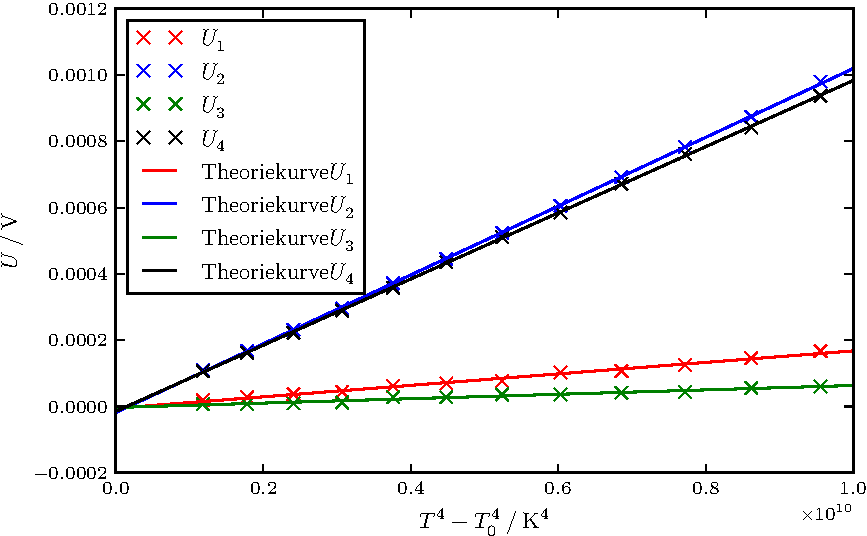
\includegraphics{plot.pdf}
  \caption{Plot zur Bestimmung des Eigenträgheitsmoments $I_{\text{D}}$ der Drillachse.}
  \label{fig:plot}
\end{figure}

Durch den Zusammenhang (\ref{eqn:zeiten}) und den Satz von Steiner \eqref{eqn:steiner},
\begin{equation}
  I_{\text{ges}} = I_{\text{D}} + (m_1+m_2)a²,
\end{equation}
folgt für die Quadrate der Umlaufzeiten
\begin{equation}
  T² = 4\pi² \frac{(m_1+m_2)}{D}a² + 4\pi² \frac{I_{\text{D}}}{D}.
\end{equation}
Folglich gilt für den aus der linearen Regression bestimmten Wert $b$,
\begin{align*}
  b = \input{build/b.tex},
\end{align*}
die Gleichung
\begin{equation}
  b = 4\pi² \frac{I_{\text{D}}}{D}
\end{equation}
und entsprechend
\begin{equation}
  I_{\text{D}} = \frac{b \cdot D}{4\pi²}.
\end{equation}
Daraus lässt sich nun die Eigenträgheit zu
\begin{align*}
  I_{\text{D}} = \input{build/eigentraegheit.tex}
\end{align*}
bestimmen.
Für die Fehlerrechnung wird bei dieser Rechnung und bei allen folgenden Rechnungen das Gaußsche Fehlerfortpflanzungsgesetz
\begin{equation}
\increment{f} = \sqrt{\Bigl(\frac{\partial f}{\partial x_1}\increment{x_1}\Bigr)^2 + \Bigl(\frac{\partial f}{\partial x_2}\increment{x_2}\Bigr)^2 + \dotsc + \Bigl(\frac{\partial f}{\partial x_n}\increment{x_n}\Bigr)^2}
\end{equation}
für eine Funktion $f(x_1,x_2, \dotsc ,x_n)$, bei der die Größen $x_1, x_2, \dotsc , x_n$ voneinander unabhängig sind, verwendet.

\subsection{Bestimmung des Trägheitsmomentes eines Zylinders}
Die Durchführung der angegebenen Messreihen für den Zylinder führt zu den in Tabelle \ref{tab:zyl} angegebenen Werten

\begin{table}[H]
  \centering
  \caption{Mesdaten zur Bestimmung des Trägheitsmomentes des Zylinders.}
  \label{tab:zyl}
  \sisetup{table-format=1.2}
  \begin{tabular}{c c c c}
    \toprule
    {$m_\text{zyl} [\si{\gram}]$} & {$r_\text{zyl} [\si{\centi\metre}]$} & {$h_\text{zyl} [\si{\centi\metre}]$} & {$T_\text{zyl} [\si{\second}]$}\\
    \midrule
    \input{build/zylindertabelle.tex}
    \bottomrule
  \end{tabular}
\end{table}

Aus diesen Messungen ergeben sich somit als Mittelwerte für die Eckdaten des Zylinders.
\begin{align*}
  R_{\text{Zylinder}} &= \input{build/r_zylinder.tex}, \\
  m_{\text{Zylinder}} &= \input{build/m_zylinder.tex}.
\end{align*}
Seine mittlere gemessene Umlaufzeit beträgt
\begin{align*}
  T_{\text{Zylinder}} = \input{build/t_zylinder.tex}
\end{align*}

Um sein theoretisches Trägheitsmoment zu bestimmen, wird die Formel für einen sich aufrechten drehenden Zylinder benutzt, welche
\begin{equation}
  I_{\text{Zylinder}} = \frac{mR²}{2}
\end{equation}
lautet.
Dementsprechend errechnet sich der theoretische Wert zu
\begin{align*}
  I_{\text{Zylinder, Theorie}} = \input{build/traegheit_zylinder_theorie.tex}. \\
\end{align*}

Aus der Gleichung (\ref{eqn:zeiten}) und nach dem Abziehen der Eigenträgheit folgt der gemessene Wert des Trägheitsmomentes zu
\begin{align*}
  I_{\text{Zylinder, gemessen}} = \input{build/traegheit_zylinder.tex}. \\
\end{align*}
Zum Theoriewert ist eine relative Abweichung nach
\begin{equation}
  \increment I = \frac{I_{\text{Zylinder, gemessen}} - I_{\text{Zylinder, Theorie}}}{I_{\text{Zylinder, Theorie}}} \cdot 100
\end{equation}
von
\begin{align*}
  \increment I = \input{build/abweichung_zylinder.tex} \:\si{\percent} \\
\end{align*}
zu erkennen.


\subsection{Bestimmung des Trägheitsmomentes einer Kugel}
Die verwendete Kugel wird auf die Größen
\begin{align*}
  R_{\text{Kugel}} &= \input{build/r_kugel.tex}, \\
  m_{\text{Kugel}} &= \input{build/m_kugel.tex}
\end{align*}
vermessen.
Wobei ihre gemessene Umlaufzeit etwa
\begin{align*}
  T_{\text{Kugel}} = \input{build/t_kugel.tex} \\
\end{align*}
beträgt.
Es ergeben sich wie zuvor beim Zylinder, jedoch mit einem Theorieträgheitsmoment nach
\begin{equation}
  I_{\text{Kugel}} = \frac{2mR²}{5},
\end{equation}
die gemessenen und errechneten Eigenschaften
\begin{align*}
  I_{\text{Kugel, Theorie}}  &= \input{build/traegheit_kugel_theorie.tex} \\
  I_{\text{Kugel, gemessen}} &= \input{build/traegheit_kugel.tex}. \\
\end{align*}
Bei jener Kugel zeichnet sich eine relative Abweichung von
\begin{align*}
  \increment I = \input{build/abweichung_kugel.tex} \:\si{\percent}\\
\end{align*}
ab.


\subsection{Bestimmung des Trägheitsmomentes einer Puppe abhängig von ihrer Pose}
Die gemittelten Maße der benutzten Holzpuppe betragen
\begin{align*}
  L_{\text{Bein1}}  &= \input{build/laenge_b_1.tex}, \\
  L_{\text{Bein2}}  &= \input{build/laenge_b_2.tex}, \\
  R_{\text{Beine}}   &= \input{build/radius_b.tex}, \\
  a_{\text{Beine}}   &= \input{build/abstand_b.tex}, \\
  L_{\text{Torso}}   &= \input{build/laenge_t.tex}, \\
  R_{\text{Torso}}   &= \input{build/radius_t.tex}, \\
  L_{\text{Kopf}}    &= \input{build/laenge_k.tex}, \\
  R_{\text{Kopf}}    &= \input{build/radius_k.tex}, \\
  L_{\text{Arme}}    &= \input{build/laenge_a.tex}, \\
  R_{\text{Arme}}    &= \input{build/radius_a.tex}, \\
  a_{\text{Arme}}    &= \input{build/abstand_a.tex}, \\
  m_{\text{ges}}     &= \input{build/masse.tex} \\
\end{align*}
wobei $L$ für Länge, $R$ für Radius, $a$ für den Abstand zur Drehachse und $m$ für die Gesamtmasse steht.
Nach ergänzen der Formel für das Trägheitsmoment auf der Seite liegender Zylinder,
\begin{equation}
  I_{\text{Zylinder}} = m \left( \frac{R²}{4} + \frac{L²}{12} \right),
\end{equation}

folgt das theoretische Trägheitsmoment in der ersten Pose zu
\begin{align*}
  I_{\text{Theorie, Pose1}}  &= \input{build/traegheit_mensch_pose_1_theorie.tex}. \\
\end{align*}
Der gemessene Wert
\begin{align*}
  T_{\text{Pose1}}  &= \input{build/t1.tex} \\
\end{align*}
führt auf ein Trägheitsmoment von
\begin{align*}
  I_{\text{gemessen, Pose1}}  &= \input{build/traegheit_mensch_pose_1.tex}. \\
\end{align*}
Die hier vorliegende prozentuale Abweichung zum Theoriewert beträgt
\begin{align*}
  \increment I  &= \input{build/abweichung_pose_1.tex}\:\si{\percent}. \\
\end{align*}

Analog folgen die Werte zur zweiten Pose durch
\begin{align*}
  T_{\text{Pose2}}  &= \input{build/t2.tex} \\
\end{align*}
auf
\begin{align*}
  I_{\text{Theorie, Pose2}}   &= \input{build/traegheit_mensch_pose_2_theorie.tex}, \\
  I_{\text{gemessen, Pose2}}  &= \input{build/traegheit_mensch_pose_2.tex}, \\
  \increment I                 &= \input{build/abweichung_pose_2.tex}\:\si{\percent}. \\
\end{align*}




%\subsection{Bestimmung des Trägheitsmomentes einer Puppe abhängig von ihrer Pose}
%Die gemittelten Maße der benutzten Holzpuppe betragen
%\begin{align*}
%  L_{\text{Bein_1}}  &= \input{build/laenge_b_1.tex}, \\
%  L_{\text{Bein_2}}  &= \input{build/laenge_b_2.tex}, \\
%  R_{\text{Beine}}   &= \input{build/radius_b.tex}, \\
%  a_{\text{Beine}}   &= \input{build/abstand_b.tex}, \\
%  L_{\text{Torso}}   &= \input{build/laenge_t.tex}, \\
%  R_{\text{Torso}}   &= \input{build/radius_t.tex}, \\
%  L_{\text{Kopf}}    &= \input{build/laenge_k.tex}, \\
%  R_{\text{Kopf}}    &= \input{build/radius_k.tex}, \\
%  L_{\text{Arme}}    &= \input{build/laenge_a.tex}, \\
%  R_{\text{Arme}}    &= \input{build/radius_a.tex}, \\
%  a_{\text{Arme}}    &= \input{build/abstand_a.tex}, \\
%  m_{\text{ges}}     &= \input{build/masse.tex} \\
%\end{align*}
%wobei $L$ für Länge, $R$ für Radius, $a$ für den Abstand zur Drehachse und $m$ für die Gesamtmasse steht.
%Nach ergänzen der Formel für das Trägheitsmoment auf der Seite liegender Zylinder,
%\begin{equation}
%  I_{\text{Zylinder}} = m \left( \frac{R²}{4} + \frac{L²}{12} \right),
%\end{equation}
%
%folgt das theoretische Trägheitsmoment in der ersten Pose zu
%\begin{align*}
%  I_{\text{Theorie, Pose_1}}  &= \input{build/traegheit_mensch_pose_1_theorie.tex}. \\
%\end{align*}
%Der gemessene Wert
%\begin{align*}
%  T_{\text{Pose_1}}  &= \input{build/t1.tex} \\
%\end{align*}
%führt auf ein Trägheitsmoment von
%\begin{align*}
%  I_{\text{gemessen, Pose_1}}  &= \input{build/traegheit_mensch_pose_1.tex}. \\
%\end{align*}
%Die hier vorliegende prozentuale Abweichung zum Theoriewert beträgt
%\begin{align*}
%  \increment I  &= \input{build/abweichung_pose_1.tex}\:\si{\percent}. \\
%\end{align*}
%
%Analog folgen die Werte zur zweiten Pose durch
%\begin{align*}
%  T_{\text{Pose_2}}  &= \input{build/t2.tex} \\
%\end{align*}
%auf
%\begin{align*}
%  I_{\text{Theorie, Pose_2}}   &= \input{build/traegheit_mensch_pose_2_theorie.tex}, \\
%  I_{\text{gemessen, Pose_2}}  &= \input{build/traegheit_mensch_pose_2.tex}, \\
%  \increment I                 &= \input{build/abweichung_pose_1.tex}\:\si{\percent}. \\
%\end{align*}


%\begin{figure}
%  \centering
%  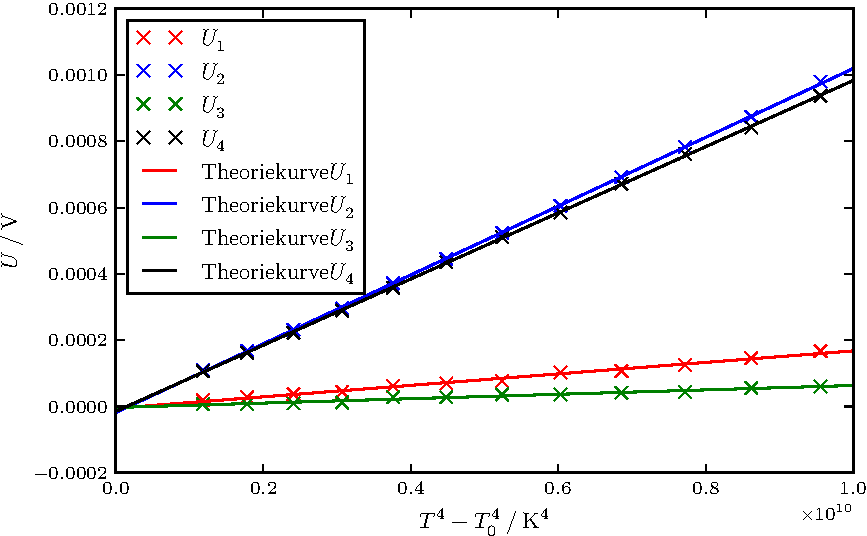
\includegraphics{plot.pdf}
%  \caption{Plot.}
%  \label{fig:plot}
%\end{figure}
%
%\begin{table}
%  \centering
%  \caption{Beispieltabelle}
%  \label{tab:tabelle_beispiel}
%  \sisetup{table-format=1.2}
%  \begin{tabular}{c c}
%    \toprule
%    {$a [\si{\second}]$} & {$b [\si{\kelvin}]$}\\
%    \midrule
%    1.0000  & 11.00 \\
2.0000  & 12.00 \\
3.0000  & 13.00 \\
4.0000  & 14.00 \\
5.0000  & 15.00 \\
6.0000  & 16.00 \\
7.0000  & 17.00 \\
8.0000  & 18.00 \\
9.0000  & 19.00 \\
10.0000 & 20.00 \\

%    \bottomrule
%  \end{tabular}
%\end{table}
%
%Es ergibt sich
%\begin{align}
%  a &= (0 \pm 0) ~ \si{\joule\per\kelvin\per\gram}
 \\
%\end{align}
%
